\section{State of the Art}
TODO
%\subsection{TODO some papers}
%

\section{Scenario Testing of AngularJS-based Single Page Web Applications}
\textcite{zhang2019scenario} present a method with the goal of achieving better undestanding of AngularJS-based \glspl{spa} and also devised a way to specify test coverage criteria based on it. At the center of the proposed method are interaction diagrams, which are used to model the overall data and control flow of an application.\parencite{zhang2019scenario}

\subsection{Abstract Syntax}
\textcite{zhang2019scenario} model a AngularJS-based \gls{spa} as a tuple ($T$, $C$, $D$, $E$), where

\begin{itemize}
  \item $T$ is a HTML template, consisting of a set of HTML tags (widgets) ($T = \{h\}$)
  \item 
  $C$ is a controller (view-model), written in JavaScript. It is modeled as a tuple ($V$, $F$, $\$scope$), where $F$ and $V$ are top level variables and functions respectively and $\$scope \in V$ is a distinguished element of $V$. Further $V(\$scope)$ and $F(\$scope)$ denote all variables and functions of $\$scope$ respectively. $W = V \setminus \{\$scope\}$ denotes top level variables not in scope. Additionally $init \in F$ is defined as an initialization function
  \item $D$ is a set of data bindings between HTML tags and variable properties of $\$scope$ $ D \subseteq \{(h,V(\$scope) \cup F(\$scope))\}$. Given $d = (n,o)$ $source(d) = n$ and $target(d) = o$. For Two-way bindings $D' \subseteq D$ and $\forall d \in D'$ $target(d) \in V(\$scope)$.
  \item $E$ a set of event handler bindings between HTML tags and function properties of $\$scope$: $E \subset \{(h,F(\$scope))\}$. In addition, for each function $f \in F \cup F(\$scope)$, $R(f) \subseteq V \cup V(\$scope)$ and $W(f) \subseteq V \cup V(\$scope)$ are defined as the values that the given function reads from and writes to. $Inv(f) \in F $ are defined as the functions invoked by $f$. \parencite{zhang2019scenario}
\end{itemize}
\subsection{Interaction Diagrams}
\label{intro:zhang_interaction_diagrams}
\textcite{zhang2019scenario} define interaction diagrams as a directed graph ($N$, $E$) where the set of nodes $N$ is defined as the union of $N_H$ (HTML tag nodes), $N_{\$scope}$ (TODO name), $N_js$ (TODO name). 

TODO double check, write as text
$N_H = \{n_h | (h,v) \in D\}$ %TODO those are html tags

$N_{\$scope} = \{n_v | (h,v) \in D\} \cup \{n_e | (h,e) \in E\} $ %(TODO those are databindings and events)

$N_js = \{n_v | v \in W\} \cup \{n_f | f \in F\} $

$n_{init}$ is distinguished by an incoming arrow without a starting vertex

Edges:

bindings 

$e_d = (target(d),source(d))$
$E_{data} = \{e_d |  d \in D \}$

addiionaly if $d \in D'$ also create $e'_t = (source(t),target(t))$ and $E'_data = \{e_d |  d \in D' \}$

for events ($E_{event}$) $(h,f) \in E$,

write $E_{W}$ $(f,v)$ where $f \in F \cup F(\$scope), v \in W(f)$

read $E_{R}$ $(v,f)$ where $f \in F \cup F(\$scope), v \in R(f)$

invoked $E_{Inv}$ $(f,v)$ where $f \in F \cup F(\$scope), v \in I(f)$


$E_{init}$ default values of widgets 
for each $h \in T $ where $ \nexists v | (h,v) \in D$ create an edge $(h,v)$ 
\
explained in a lot of detail in \parencite[9]{zhang2019scenario}

\subsection{Testing and Interactions}
%TODO ... the red text p10
\textcite{zhang2019scenario} define an interaction as a round of user input including updates to the widgets by the application. Interaction can be triggered explicitly by the user (by invoking an event handler) or implicitly while the user is updating data. \parencite{zhang2019scenario} %TODO anton I don't model it like ths, don't need

Given the interaction diagrams as described in \ref{intro:zhang_interaction_diagrams} it is possible to derive which widgets get updated by a user input action or set up by the initial function. \textcite{zhang2019scenario} define it formally as follows:
\begin{quote}
\label{quote:interactions}
Given a node $n \in N_H \cup \{init\}$, we say a node $m \in N_H$ \textit{reacts} to $n$ iff
  \begin{enumerate}
      \item $\exists n_0,n_1,n_2, \ldots,n_k \in N, n_0=n,n_k=m$ such that for each $0 \leq i < k  $ $(n_i,n_{i+1}) \in E$, and 
      \item $\forall n_p, 1 < p \leq k$ and $\forall e \in E, target(e)= n_p$ it holds that $e \notin E_{event}$  
  \end{enumerate}
  We write $l(n)$ for the set of all nodes representing the widgets that react to $n$. This set contains the widgets that are automatically updated upon user input,
  and thus constitute an interaction.
  \end{quote}

For example, in order for the widget $n$, which was clicked by the user, to update the widget $m$, $m$ must be reachable from $n$ by following the directed edges of the interaction diagram and only the first edge can be an event-handling edge.

What is crucial is that the interactions $l(n)$ define an upper bound of what can be updated, i.e. what might get updated. Nevertheless, this information is sufficient in order to be able to define coverage criteria \parencite{zhang2019scenario}.

\subsection{Coverage Criteria}
Interactions should not be tested in isolation and in order for tests to make sence, interactions as preconditions are required \parencite{zhang2019scenario}. 
In order to define coverage criteria, \textcite{zhang2019scenario} extend their notation, as described in \ref{intro:zhang_interaction_diagrams}, by defining - $\mathcal{I}  = \{w\in T | l(w) \neq \emptyset \}$ all widgets, that result updates.

A sequence of user interactions, including the initial function is refered to as a \textit{scenario} $A=(a_0,a_1,\ldots, a_n)$ where $a_0=init$ and $\forall0 < k \leq n, a_k \in \mathcal{I}$. The widgets, to which a scenario reacts, are equal to the widgets to which the last widget in the scenario reacts - $l(A)=l(a_n)$. 


The set of scenarios is generated by starting with the initial scenario, containing only the initial function $S_0 = \{(init)\}$ and prolonging it iteratively by each widget, where the user can take an action. This is terminated once all $i \in \mathcal{I}$ are included in at least one scenario. Formally:
Define $A \oplus x = a_0,a_1,\ldots,a_n,x$ For $n > 0, S_{n+1}= \{ p \oplus x |p \in S_n, x \in l(p) \cap \mathcal{I}\}$ 

Based on the scenario sets \textcite{zhang2019scenario} define the following coverage criteria:
\begin{quote}
  

\begin{itemize}
  \item Each set $S_n$ of test scenarios should be tested.
  \item For each given $S_n$, each $p \in S_n$ should be tested.
  \item For each given $p$, each $w \in l(p)$ should be tested. That is, there should be a
  test case for each widget that may be modified after the scenario $p$.
\end{itemize} 
\end{quote}

\section{Scenario Testing}
Scenario testing, was originally introduced in \textcite{kaner2003power} and later as \textcite{kaner2013introduction}. The author defines scenarios as hypothetical stories, which aid a person in understanding a complex system or problem. Scenario tests are tests, which are based on such scenarios.  \parencite[1]{kaner2013introduction}
Further, \parencite[2-5]{kaner2003power} defines five characteristics, which make up a good scenario test as follows:
A Scenario test must be
\begin{itemize}
     \item based on a story - based on a description of how the program is being used
    \item motivating - stakeholders have interest in this test succeeding and would see to it's resolution
    \item credible - probable to happen in the real world
    \item complex - complex use, data or environment
    \item easy to evaluate - it should be easy to tell if the test succeded or failed based on the results 
\end{itemize}

\textcite{kaner2013introduction} describes the biggest advantages of scenario testing to be  - understanding and learning the product in early stages of development(1), connecting of testing and requirement documentations(2), exposing shortcomings in delivering of desired benefits(3), exploration of expert use of the program(4), expose requirement related issues(5).

\section{Behavior-Driven Development}
Behavior-Driven Development (BDD), pioneered by  \textcite{north2006behavior} is a software development
process , that combines principles from Test-Driven Development and Domain-Driven design \parencite{evans2004domain}.

Its main goal is to specify a system in terms of its functionality (i.e. it's behaviors) with a simple domain-specific language (DSL) making use of English-like sentences. This stimulates collaboration between developers and non-technical stakeholders and further results in a closer connection between acceptance criteria for a given function and matching tests used for its validation.

BDD splits a user story into multiple scenarios, each formulated in the form of \textit{Given}, \textit{When}, \textit{Then} statements, respectively specifying the prerequisite/context, event and outcomes of a scenario. 

[TODO] example here? cut shorter

At present ... there based on the division of behavior descriptions and behaviors. Such as Jest/Jasmine combine behavior descriptions and behaviors into one, whereas as Cucumber uses a DSL named Gherkin to specify the behavior descriptions and provides a set of tools to generate behaviors.
%[TODO example A vs B? ]


% \subsection{the other one(forgot name)}
% splitting into ...
\subsection{Gherkin Language}

\section{Model-View-ViewModel}
\label{sec:mvvm}
\gls{mvvm} is a design pattern, which helps in creating a clear separation between business and presentation logic and \gls{ui} of an application. \parencite[7-9]{microsoft_mvvm}

In \gls{mvvm} there are three core components - the view, model and view model. Those components are clearly separated from each other - the view is aware of the view model and the view model is aware of the model. However, this does not hold in reverse - the model is unaware of the view model and the view model is unaware of the view. 

\begin{figure}[H]
  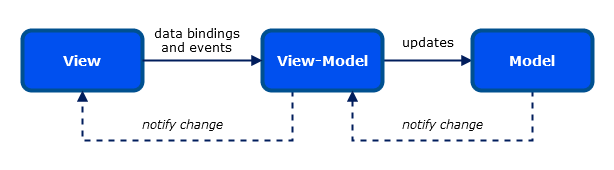
\includegraphics[width=\textwidth]{images/mvvm.png}
   \caption{\gls{mvvm} design pattern overview, adapted from \parencite[7]{microsoft_mvvm}}
   \label{fig:mvvm}
 \end{figure}

\subsection{View}
The view is what the user sees. It is responsible for the structure, layout and appearance of the application.
\subsection{View-Model}
The view model implements event handlers and properties, to which the view can bind to. It also notifies the view of any changes to the underlying data. It defines the functionality, offered by the \gls{ui}, but the view determines how it is presented. 
\subsection{Model}
The model encapsulates the data of the application and validation its logic.


\section{Vue.js}

Vue.js \parencite{vuejs_gh} is a progressive front end framework for building user intefaces and single-page applications based on the \gls{mvvm} design pattern described in \ref{sec:mvvm} \parencite{vuejs_book} \parencite{vuejs_guide}.  

\subsection{Components}
At the core of Vue.js are components, which are small, self-contained, composable and often reusable custom elements. Almost any type of application can be represented as a tree of components \parencite{vuejs_guide}. 

In more concrete terms, a Vue.js component is a single file with the extension of \code{.vue}, which consists of a \code{template}, \code{script} and optional \code{style} part. The \code{template} is a HTML-based template, which can be parsed specification compliant browsers and HTML parsers. It can contain other components or html elements and is equivalent to the \textit{view} in \gls{mvvm}. 

The \textit{code} section of a Vue.js component includes the view-model of the component. It has a special json object \code{data}, which is equivalent to the \gls{mvvm} model. %TODO not so nicely written
The \code{script} part of a computed includes css-like styles.


data binding is a general technique that binds data sources from the provider and consumer together and synchronizes them.


\subsection{Reactivity}

%TODO this with own words here
% https://vuejs.org/v2/guide/reactivity.html

\dots enables data binding
\subsection{Directives}
Vue.js enables one way bindings(from source - data to target - component or html tag) via the \code{v-bind} (line X,Y) or \textit{moustache} syntax (line Z). 
Bindings can contain expressions (line X,Y). 

Two way binding can be achieved using the \textit{v-model} directive (line,X,Y,Z). 
Event handlers can be bound by the method name or also expressions.

%TODO vfor binding here

%TODO examples in code snippet image

\subsection{Data Binding}
Vue.js provides support for various forms of \gls{databinding} via a special syntax. Both the data and computed objects of a \code{Vue.js} component are reactive 


Via a special syntax
\code{Vue.js}
- one way
- two way
- event bindings
- inline expressions
- computed properties

\subsection{Vue.js directives}
\subsection{Structure of a Component}

(template, code etc.)

bindings two way, one way

g
- data
- computed properties

template part
code part
bindings


\section{ESLint}

ESLint \parencite{eslintMainPage} is a linting tool (linter) for ECMAScript/JavaScript. Linters are static code analysis tool, which can be used to flag and potentially automatically fix common code issues and enforce consistent code styling.

\subsection{Rules}
At the core of ESLint are rules. Rules are extensible pieces of code, bundled as plugins, which can be used to verify various aspects of code. An example would be a rule, which checks for matching closing paranthesis. 
Each rule consists of a \code{metadata} object
and a \code{create} function. The metadata object includes metadata such as documentation strings, the type of the rule and whehter it is fixable or not.

Based on type, rules can be either \textit{suggestions}, \textit{problems} or \textit{layout}. Suggestions indicate some improvement, but are not required and would not cause the linting to fail. Problems on the other hand would result in a linting failure. Layouts are rules that care mainly about the formatting of code, such as whitespaces, semicolons, etc. 

If the fixable property is specified, it indicates that the errors reported by this rule can be automatically fixed. This can be applied via the \code{--fix} command line option. It has two possible values - \textit{code} or \textit{whitespace} indicating the type of fixes, that this rule would apply. For example in \glspl{ide} fixable \textit{code} errors would show a fix shortcut displayed next to them and \textit{whitespace} rules could be applied when saving the file.

The \code{create} function of rules takes as arguments a \code{context} and returns an object of methods which are called by ESLint for each node based on the \gls{visitor} pattern while traversing the \gls{ast}. 

\subsection{Selector}
ESLint provides a very powerful matching mechanism for specifying what nodes to match called selectors \parencite{eslintSelectors} inspired by \textcite{estoolsEsQuery}.

Some selectors include:
\begin{itemize}
  \item AST Nodes - \code{MemberExpression} matches any node of type \code{MemberExpression}
  \item descendant -  \code{MemberExpression Identifier} matches any node of type \code{Identifier} who has a descendant of type \code{MemberExpression} in the tree
  \item child - \code{MemberExpression > Identifier} matches any node of type \code{Identifier} who has a direct parent (is a child of) of type \code{MemberExpression}
  \item :not -\code{:not(MemberExpression)} negation of a selector. In this case, matches any node, that is not a \code{MemberExpression} node
  \item :matches - \code{:matches(MemberExpression, Identifier)} matches any of the selectors. In this case, either a \code{MemberExpression} or \code{Identifier}.
  \item attributes - \code{Property[name=a]}. Matches any AST Node, whose specified attribute has the specified value.
\end{itemize}

\subsection{AST Explorer}
An incredibly useful tool when working with \glspl{ast} is \gls{ast} Explorer, developed by \textcite{astexplorer_fkling2021Jan}. It enables the exploration of syntax tree generated by various parsers and also includes the vue-eslint-parser \parencite{eslint_vue_parser}

\subsection{ESTree AST}
By default ESLint uses the \parencite{eslintEspree} parser to parse JavaScript source code into an \gls{ast} as defined by ESTree specification \parencite{estreeASTSpec}. When Parsing \textit{.vue} files ESLint uses this parser for the code inside the \code{<script>} tag.
  
\subsection{ESLint Parser Vue AST}
In order to parse the \code{<template>} section of \textit{.vue} files, ESLint uses the vue-eslint-parser \parencite{eslint_vue_parser}. This parser outputs an  \gls{ast} compliant with their own  \gls{ast}specification, defined in \parencite{eslint_vue_parser_ast}.


%TODO compound graph? directed graph?


%TODO does AST need explaining?